\chapter{Evaluación del modelo}
\label{chap:evaluacion}
Recordemos que el problema que buscamos resolver a través de este modelo es el de priorizar correctamente las verificaciones domiciliarias, reduciendo así la proporción de hogares que son sujetos a un proceso de focalización incorrecta. Dada la deriva temporal a la que está sujeto el proceso de focalización -los programas que operan en cierta región, así como los criterios que utilizan para focalizar, están cambiando constantemente- simplificamos el problema al definir que nuestro objetivo es, simplemente, asignar correctamente las verificaciones. Definimos como una verificación correctamente asignada a aquella en la que se tuvo que corregir el valor de al menos una variable. Así, podemos utilizar la distribución posterior resultante de nuestro modelo bayesiano para definir un clasificador que indique una verificación a realizar en caso de que haya una probabilidad de tener cambios suficientemente alta.
\par
\noindent
Podemos entonces comparar entre conjuntos de variables como comparamos entre clasificadores. Sin embargo, dado un conjunto de variables, necesitamos escoger el valor de $k$ que resulte en la estructura más adecuada. Definimos entonces nuestro proceso de evaluación de modelos en dos pasos.
\section*{Comparación de estructuras}
Lo primero que necesitamos asegurar es que, dado un conjunto de variables, tenemos la mejor estructura posible que el algoritmo sea capaz de encontrar. Necesitamos escoger entonces una medida de bondad de ajuste para la distribución conjunta inducida por la estructura de la gráfica.
\par
\noindent
Dado que escogimos un modelo bayesiano, resulta natural pensar en la verosimilitud -o alguna transformación monótona de esa función- para evaluar modelos. En nuestro caso, decidimos utilizar la devianza de prueba por la facilidad de interpretarla de forma análoga a la suma de cuadrados residuales, en el caso de regresión lineal por mínimos cuadrados\foonote{Es decir, que una devianza de validación en el modelo "perfecto" o saturado es igual a cero, y la devianza de validación incrementa conforme el ajuste del modelo empeora}. La devianza de prueba para un modelo $M_0$, que estima $\hat{\mu} := E[Y|\hat{\theta}_0]$ basada en las observaciones $y$ está definida por:
\begin{align*}
D(y, \hat{\mu}) &= 2(log(p(y|\hat{\theta}_s)) - log(p(y|\hat{\theta}_0)))
\end{align*}
Donde $\hat{\theta}_0$ denota los valores de los parámetros del modelo a evaluar $M_0$, y $\hat{\theta}_s$ denota los valores de los parámetros del modelo \textbf{saturado}. Esta métrica nos permite, dado un conjunto de variables, escoger el valor de $k$ que nos dé la mejor estructura posible para minimizar la devianza.
\par
\noindent
Después de un poco de exploración con las restricciones, decidimos considerar los siguientes seis modelos:
\begin{enumerate}
\item \textbf{Modelo sin restricciones}: modelo que incluye solamente las variables reportadas y verificadas, sin ninguna restricción para el algoritmo de búsqueda de estructura.
\item \textbf{Modelo base}: modelo que incluye solamente las variables reportadas y verificadas, con la restricción de que no exista una arista de una variable reportada a una verificada.
\item \textbf{Modelo base + variables municipales}: modelo base con las variables a nivel municipal que componen el índice de marginación de CONAPO.
\item \textbf{Modelo base + GM}: modelo base con la variable de grado de marginación: una discretización del índice de marginación a través del método Dalenius.
\item \textbf{Modelo base + variables municipales + GM}: modelo base con la variable de grado de marginación y con todas las variables que lo componen.
\item \textbf{Modelo base + 3 variables municipales}: modelo base con tres variables a nivel municipal: analfabetismo, falta de drenaje/excusado y hacinamiento.
\end{enumerate}
Utilizando la métrica propuesta, comparamos cada uno de los modelos para escoger el mejor valor del parámetro de regularización. Los resultados preliminares son los siguientes:
\begin{figure}[h]
    \caption{Devianza de validación para todos los modelos considerados. Dado que la razón de verosimilitud tiene un denominador distinto (estamos considerando distintos conjuntos de variables), no es comparable entre gráficas}
    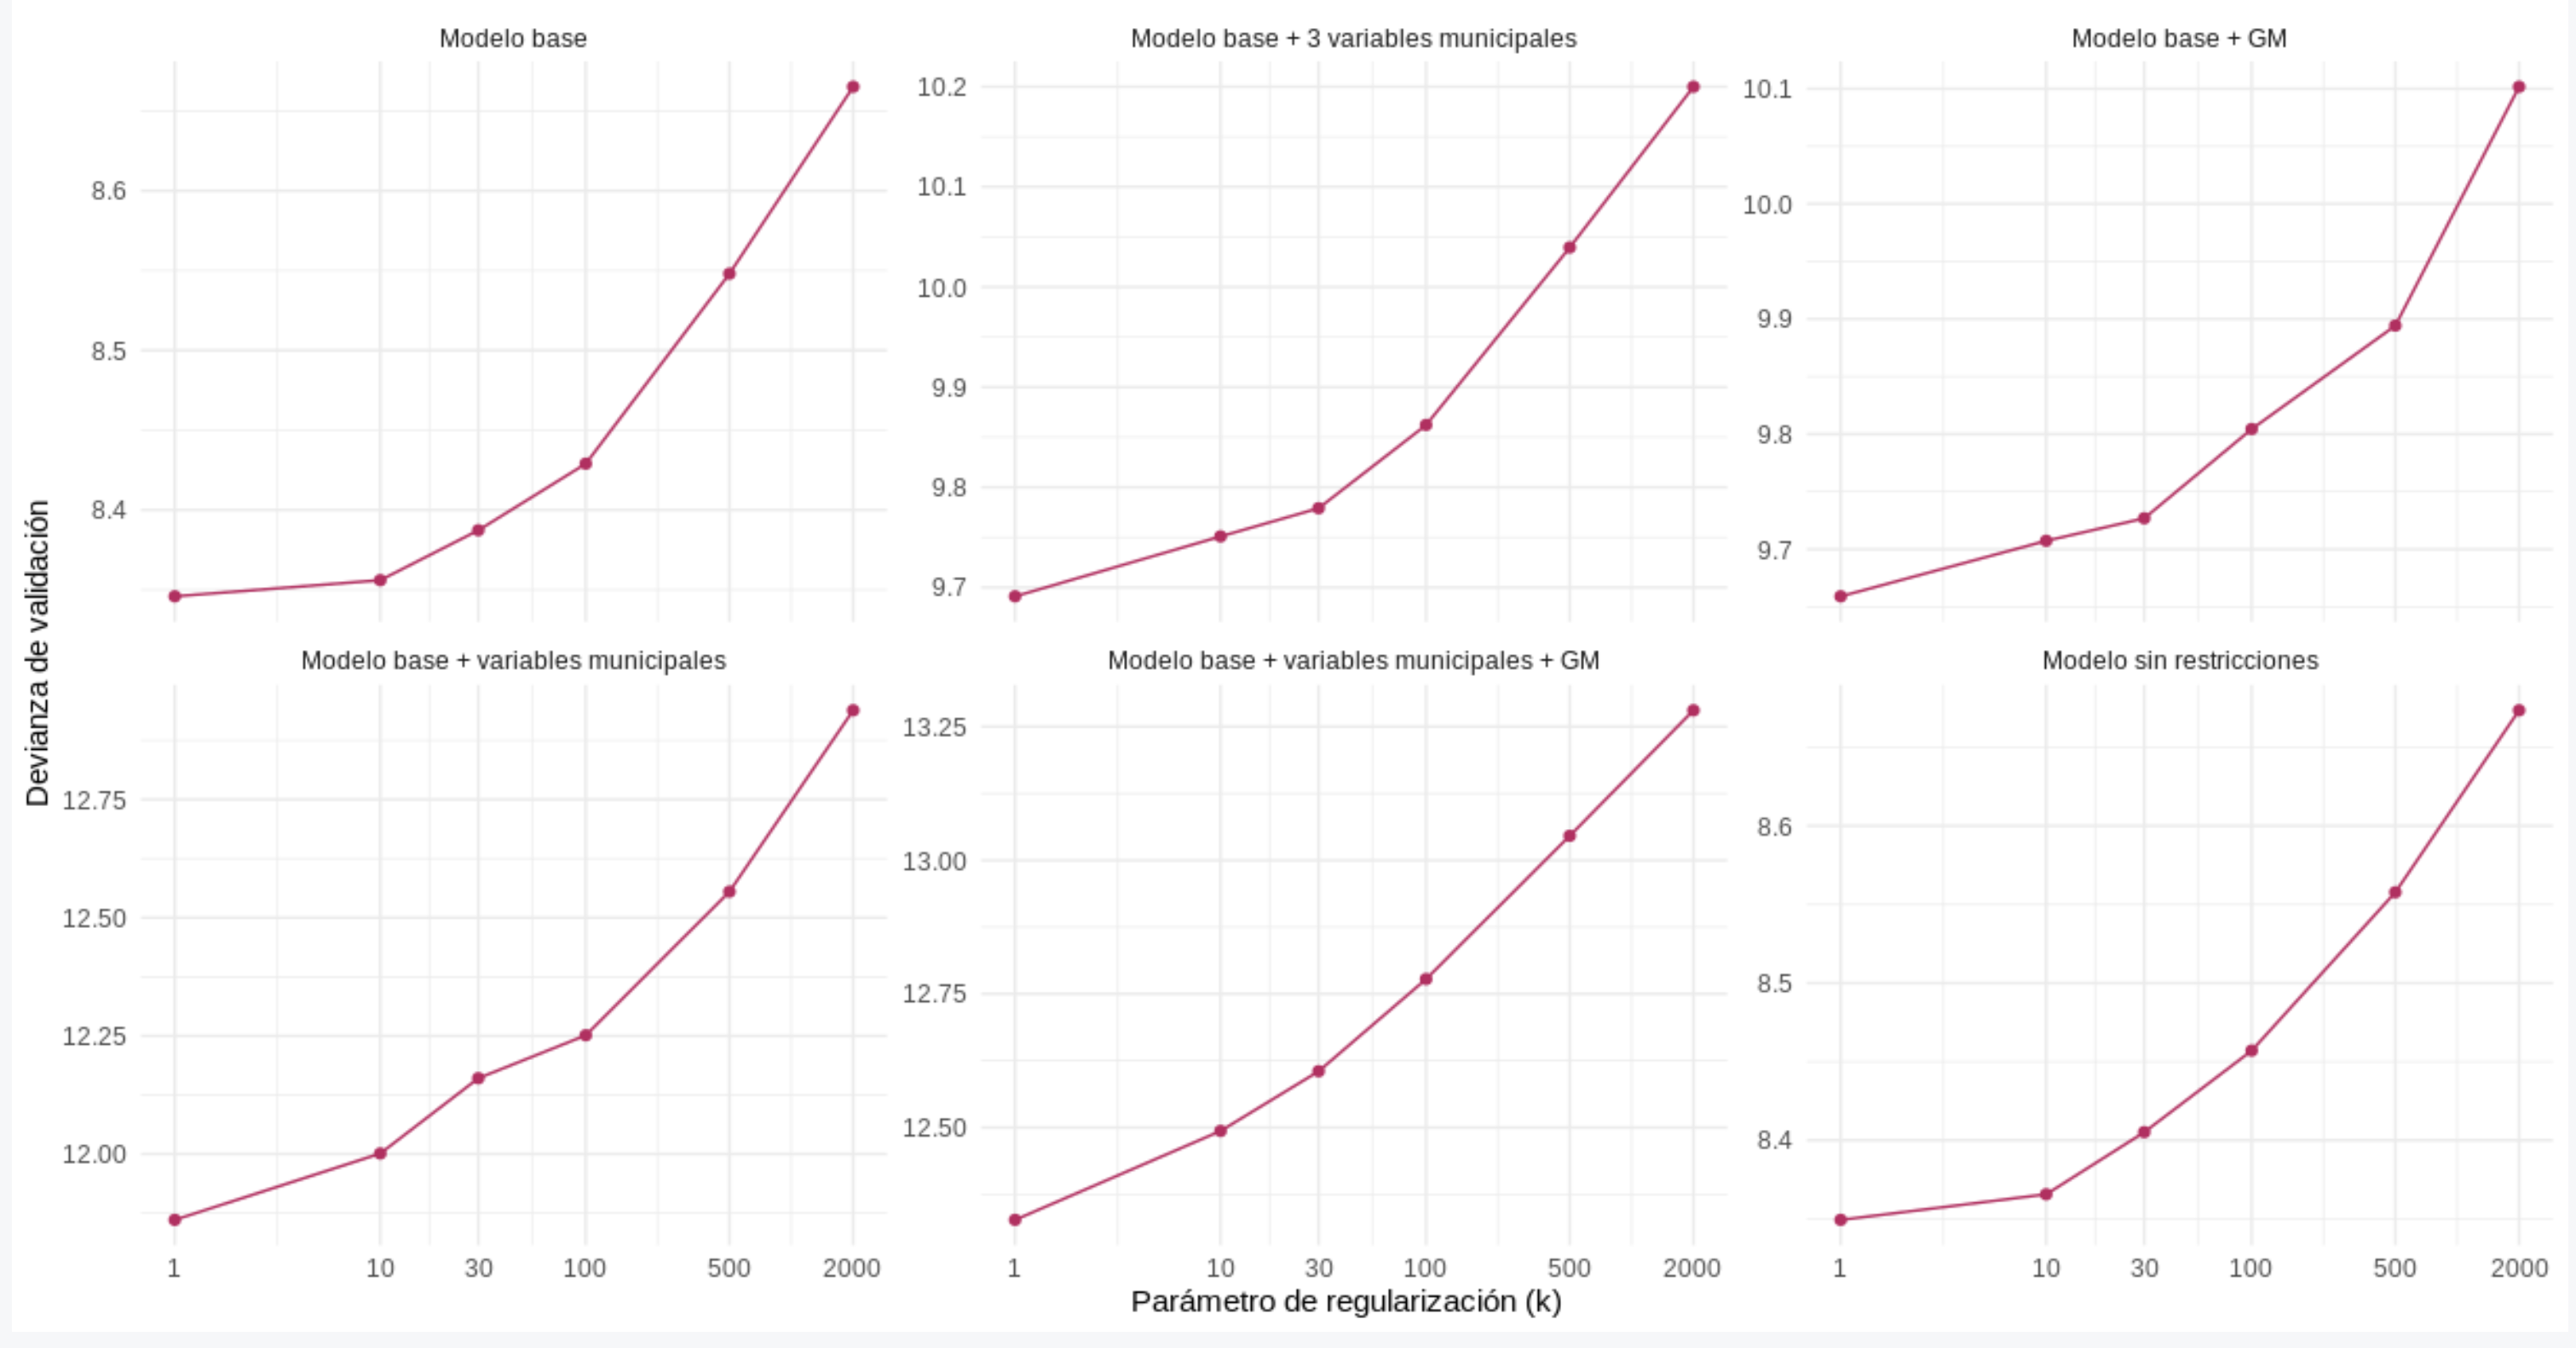
\includegraphics{devianza_validacion.png}
\end{figure}
\section*{Comparando distintos conjuntos de variables}
Una vez que escogimos la mejor estructura posible dado un conjunto de variables, es necesario construir el clasificador que mencionamos anteriormente. Necesitamos entonces hacer inferencia probabilística para obtener un estadístico que nos ayude con la tarea de clasificación.
\par
\noindent
Existen varios métodos de inferencia para Redes Bayesianas. Nosotros consideramos dos métodos de inferencia:
\begin{enumerate}
    \item
\end{enumerate}

Entonces, lo que hacemos es revisar cómo le va a distintos cortes de la suma de probabilidades y así construir un clasificador discreto. Por lo tanto, tiene sentido evaluarlo con funciones como la curva ROC y el AUC.
\subsection*{Métodos de imputación}
\subsection*{Proceso de clasificación}
Definir la curva ROC y el AUC. Explicar cómo se calcula en un contexto como este, con polinomios de Newton.

